\documentclass[tikz,border=2pt]{standalone}
\usepackage{amsmath,amssymb}
\usepackage{tikz}

\begin{document}
% Sample paths of X_n = 1{U < 1/n} for three outcomes of U: each path is 1 only while n < 1/U
% and 0 from then on, so every path with U > 0 converges to 0.
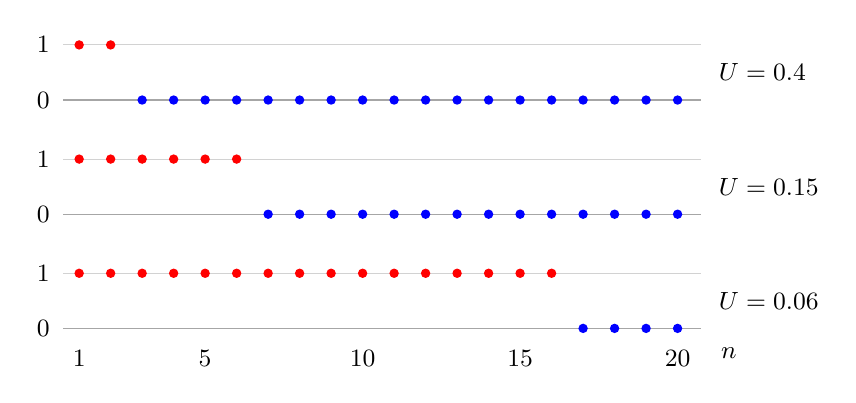
\begin{tikzpicture}[every node/.style={font=\small}]
	\foreach \row/\u/\last in {0/0.4/2, 1/0.15/6, 2/0.06/16} {
		\pgfmathsetmacro{\yb}{-1.45*\row}
		\pgfmathsetmacro{\yt}{-1.45*\row+0.7}
		\pgfmathsetmacro{\ym}{-1.45*\row+0.35}
		\draw[gray!70] (0.2,\yb) -- (8.3,\yb);
		\draw[gray!35] (0.2,\yt) -- (8.3,\yt);
		\node[anchor=east, font=\small] at (0.15,\yb) {$0$};
		\node[anchor=east, font=\small] at (0.15,\yt) {$1$};
		\foreach \n in {1,...,20} {
			\ifnum\n>\last
				\fill[blue] (0.4*\n,\yb) circle (1.7pt);
			\else
				\fill[red] (0.4*\n,\yt) circle (1.7pt);
			\fi
		}
		\node[anchor=west, font=\small] at (8.4,\ym) {$U=\u$};
	}
	\foreach \n in {1,5,10,15,20} {
		\node[anchor=north, font=\small] at (0.4*\n,-3.05) {$\n$};
	}
	\node[anchor=north, font=\small] at (8.65,-3.02) {$n$};
	
\end{tikzpicture}
\end{document}
